\documentclass[t]{beamer}
\usepackage[T1]{fontenc}
\usepackage[utf8]{inputenc}
\usepackage{lmodern}
\usepackage[ngerman]{babel}
\usepackage{caption}

\newcommand{\beamerred}{\usebeamercolor[fg]{frametitle}}
\newcommand{\beamerblue}{\usebeamercolor[fg]{description item}}

\setbeamertemplate{section in toc}{\hspace*{1em}{\beamerred \inserttocsectionnumber.~\inserttocsection}\par}
\setbeamertemplate{subsection in toc}{\hspace*{2em}\inserttocsectionnumber.\inserttocsubsectionnumber~\inserttocsubsection\par}

\beamertemplatenavigationsymbolsempty
\useoutertheme{infolines}
\usecolortheme{beaver}
\setbeamertemplate{headline}{}

\title{Projektpräsentation: Subgraph isomorphisms}
\author{Team SPUNIKNSS15}
\date{}
\titlegraphic{\vspace{-0.8cm}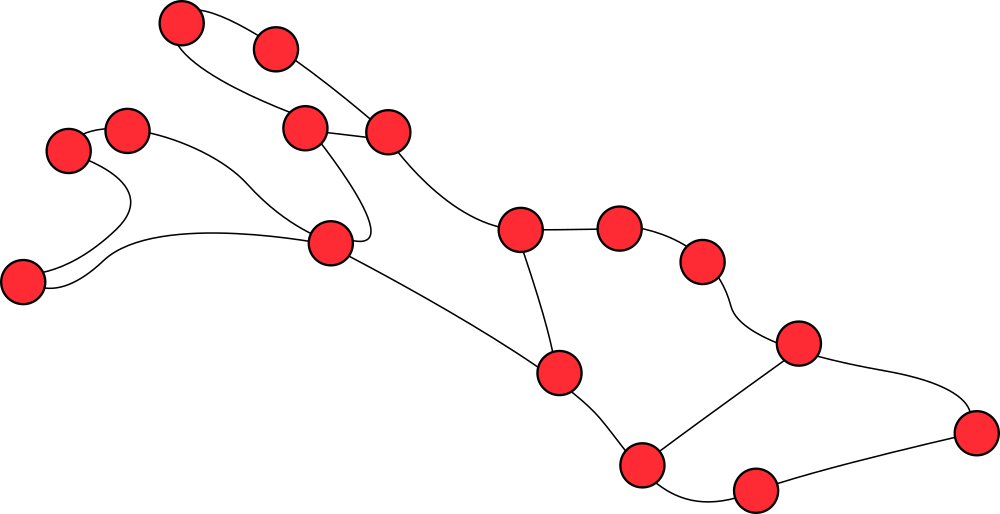
\includegraphics[width=\textwidth]{../../Logo/logo_no_text.png}}

\begin{document}
  \frame{
  \titlepage
}

  \frame{
    \tableofcontents
  }
  \section{Funktionsweise von ISGCI und VF2}
  \newcommand{\hl}[1]{\textbf{\LARGE#1}}

\begin{frame}{{\it\hl{I}{\large nformation} \hl{S}{\large ystem on} \hl{G}{\large raph}
  \hl{C}{\large lasses and their} \hl{I}{\large nclusions}}\\Aufbau und Funktionalität}{}
	\begin{itemize}
	  \item Java Projekt zur Entdeckung und Analyse von Beziehungen zwischen Graph-Klassen
	  \item Relevant für unser Projekt:
	  \begin{itemize}
	    \setlength\itemsep{1em}
	    \item {\tt teo.isgci.smallgraph}: Implementierung von Smallgraphs, Configurations, Families
	    \item {\tt smallgraphs.xml}: Große Sammlung von Smallgraphs, Configurations, Families
	    \item {\tt teo.isgci.appl.FindISG}: Applikation zum Finden induzierter Subgraphen von
	      Konfigurationen und Familien. \\
	      Resultat: {\tt output.xml}
	  \end{itemize}
	\end{itemize}
\end{frame}

  \begin{frame}{Der VF2 Algorithmus}{}
	\begin{itemize}
	  \item VF2: \\
	    \( (G_1, G_2) \mapsto \begin{cases}
                              \texttt{True},~~ \textit{\small falls \(G_2\) isomorph zu induz. Subgraph von \(G_1\)} \\
                              \texttt{False},~~ \textit{\small sonst}
                            \end{cases}\)
	  \item VF2 ist
	    \begin{itemize}[]
	      \item<.-> allgemein
	      \item<.-> vergleichsweise effizient
	      \item<.-> und erlaubt semantische Matchings
	    \end{itemize}
	    \textit{(Cordella, Foggia, Sansone, Vento)}.
	\end{itemize}
	\begin{figure}
	  \centering
    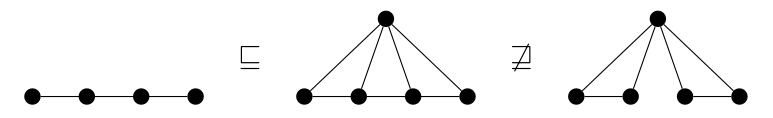
\includegraphics[width=0.7\textwidth]{subisomorphie.png}
	\end{figure}
\end{frame}

  \section{Projektablauf}
    

    \subsection{Lange Analysephase}
    \input{analysephase}
    \subsection{Teamaufteilung}
    \begin{frame}{Organisation}{}
	\begin{itemize}
	  \large
	  \setlength\itemsep{1em}
	  \item Zwei getrennte Aufgabenfelder: \texttt{ISGCI} und \texttt{VF2} \\
	  \item Deshalb: Aufteilung des Teams und der Milestones
	  \begin{itemize}[]
	    \setlength\itemsep{1em}
	    \large
	    \item {\bf \beamerblue Milestone 1:} Implementierung des \texttt{VF2}-Algorithmus
	    \item {\bf \beamerblue Milestone 2:} Ersetzung der Adjazenzmatrizen in \texttt{ISGCI} durch
	      \texttt{jgrapht}-Objekte
	    \item {\bf \beamerblue Milestone 3:} Integration des \texttt{VF2} in \texttt{ISGCI}
	  \end{itemize}
	\end{itemize}
\end{frame}

    \subsection{Trennung der Milestones (??)}
    \input{milestones}
    \subsection{Reflektion}
    \begin{frame}{Herausforderungen}{}
  \Large
	\begin{enumerate}
	  \item Analysephase
	  \item Teamkoordination
	  \item Tools
	\end{enumerate}
\end{frame}

    \subsection{Extras}
    \input{extras}
  \section{Laufzeit}
  \renewcommand{\mark}[1]{\node[circle,fill=#1] {};}

\begin{frame}[<+->]{Laufzeit von \texttt{FindISG} - (1)}{}
  {\beamerblue Vor unseren Änderungen.\newline}
  \begin{figure}
    \centering
    \begin{tikzpicture}
  \matrix (m) [matrix of nodes,ampersand replacement=\&] {
\mark{black} \& \mark{black} \& \mark{black} \& \mark{black} \& \mark{black} \& \mark{black} \& \mark{black} \& \mark{black} \& \mark{black} \& \mark{black}\\
\mark{black} \& \mark{black} \& \mark{black} \& \mark{black} \& \mark{black} \& \mark{black} \& \mark{black} \& \mark{black} \& \mark{black} \& \mark{black}\\
\mark{black} \& \mark{black} \& \mark{black} \& \mark{black} \& \mark{black} \& \mark{black} \& \mark{black} \& \mark{black} \& \mark{black} \& \mark{black}\\
\mark{black} \& \mark{black} \& \mark{black} \& \mark{black} \& \mark{black} \& \mark{black} \& \mark{black} \& \mark{black} \& \mark{black} \& \mark{black}\\
\mark{black} \& \mark{black} \& \mark{black} \& \mark{black} \& \mark{black} \& \mark{black} \& \mark{black} \& \mark{black} \& \mark{black} \& \mark{black}\\
\mark{black} \& \mark{black} \& \mark{black} \& \mark{black} \& \mark{black} \& \mark{black} \& \mark{black} \& \mark{black} \& \mark{black} \& \mark{black}\\
\mark{black} \& \mark{black} \& \mark{black} \& \mark{black} \& \mark{black} \& \mark{black} \& \mark{black} \& \mark{black} \& \mark{black} \& \mark{black}\\
\mark{black} \& \mark{black} \& \mark{black} \& \mark{black} \& \mark{black} \& \mark{black!50!white} \& \mark{black!50!white} \& \mark{black!50!white} \& \mark{black!50!white} \& \mark{black!50!white}\\
\mark{black!50!white} \& \mark{black!50!white} \& \mark{black!50!white} \& \mark{black!50!white} \& \mark{black!50!white} \& \mark{black!50!white} \& \mark{black!50!white} \& \mark{black!50!white} \& \mark{black!50!white} \& \mark{black!50!white}\\
\mark{black!50!white} \& \mark{black!50!white} \& \mark{black!50!white} \& \mark{black!50!white} \& \mark{black!50!white} \& \mark{black!50!white} \& \mark{black!50!white} \& \mark{black!50!white} \& \mark{black!50!white} \& \mark{black!50!white}\\
};
\end{tikzpicture}

  \end{figure}
  \begin{center}
    
\includegraphics[width=0.4cm]{stop-watch-icon.png} \bf ~~~ 150 Minuten
  \end{center}
\end{frame}

\begin{frame}[<+->]{Laufzeit von \texttt{FindISG} - (2)}{}
  {\beamerblue Verwendung der ersten Version des Java-VF2 anstelle der C++ Version.\newline}
  \begin{figure}
    \centering
    \begin{tikzpicture}
  \matrix (m) [matrix of nodes,ampersand replacement=\&] {
    \mark{black!50!white} \& \mark{black!50!white} \& \mark{black!50!white} \& \mark{black!50!white} \& \mark{black!50!white} \& \mark{black!50!white} \& \mark{black!50!white} \& \mark{black!50!white} \& \mark{black!50!white} \& \mark{black!50!white}\\
    \mark{black!50!white} \& \mark{black!50!white} \& \mark{black!50!white} \& \mark{black!50!white} \& \mark{black!50!white} \& \mark{black!50!white} \& \mark{black!50!white} \& \mark{black!50!white} \& \mark{black!50!white} \& \mark{black!50!white}\\
    \mark{black!50!white} \& \mark{black!50!white} \& \mark{black!50!white} \& \mark{black!50!white} \& \mark{black!50!white} \& \mark{black!50!white} \& \mark{black!50!white} \& \mark{black!50!white} \& \mark{black!50!white} \& \mark{black!50!white}\\
    \mark{black!50!white} \& \mark{black!50!white} \& \mark{black!50!white} \& \mark{black!50!white} \& \mark{black!50!white} \& \mark{black!50!white} \& \mark{black!50!white} \& \mark{black!50!white} \& \mark{black!50!white} \& \mark{black!50!white}\\
    \mark{black!50!white} \& \mark{black!50!white} \& \mark{black!50!white} \& \mark{black!50!white} \& \mark{black!50!white} \& \mark{black!50!white} \& \mark{black!50!white} \& \mark{black!50!white} \& \mark{black!50!white} \& \mark{black!50!white}\\
    \mark{black!50!white} \& \mark{black!50!white} \& \mark{black!50!white} \& \mark{black!50!white} \& \mark{black!50!white} \& \mark{black!50!white} \& \mark{black!50!white} \& \mark{black!50!white} \& \mark{black!50!white} \& \mark{black!50!white}\\
    \mark{black!50!white} \& \mark{black!50!white} \& \mark{black!50!white} \& \mark{black!50!white} \& \mark{black!50!white} \& \mark{black!50!white} \& \mark{black!50!white} \& \mark{black!50!white} \& \mark{black!50!white} \& \mark{black!50!white}\\
    \mark{black!50!white} \& \mark{black!50!white} \& \mark{black!50!white} \& \mark{black!50!white} \& \mark{black!50!white} \& \mark{black!50!white} \& \mark{black!50!white} \& \mark{black!50!white} \& \mark{black!50!white} \& \mark{black!50!white}\\
    \mark{black!50!white} \& \mark{black!50!white} \& \mark{black!50!white} \& \mark{black!50!white} \& \mark{black!50!white} \& \mark{black!50!white} \& \mark{black!50!white} \& \mark{black!50!white} \& \mark{black!50!white} \& \mark{black!50!white}\\
    \mark{black!50!white} \& \mark{black!50!white} \& \mark{black!50!white} \& \mark{black!50!white} \& \mark{black!50!white} \& \mark{black!50!white} \& \mark{black!50!white} \& \mark{black!50!white} \& \mark{black!50!white} \& \mark{black!50!white}\\
  };
  \node {\textcolor{red}{\Huge \(\infty\)}};
\end{tikzpicture}

  \end{figure}
  \begin{center}
    
\includegraphics[width=0.4cm]{stop-watch-icon.png} \bf ~~~ über 12 Stunden
  \end{center}
\end{frame}

\begin{frame}[<+->]{Laufzeit von \texttt{FindISG} - (3)}{}
  {\beamerblue Weglassen der Erzeugung sämtlicher Subgraphen, stattdessen direkter Test
   auf Subisomorphie.}
  \begin{figure}
    \centering
    \begin{tikzpicture}
  \matrix (m) [matrix of nodes,ampersand replacement=\&] {
\mark{black} \& \mark{black} \& \mark{black} \& \mark{black} \& \mark{black} \& \mark{black} \& \mark{black} \& \mark{black} \& \mark{black} \& \mark{black}\\
\mark{black} \& \mark{black} \& \mark{black} \& \mark{black} \& \mark{black} \& \mark{black} \& \mark{black} \& \mark{black} \& \mark{black} \& \mark{black}\\
\mark{black} \& \mark{black} \& \mark{black} \& \mark{black} \& \mark{black} \& \mark{black} \& \mark{black} \& \mark{black} \& \mark{black} \& \mark{black}\\
\mark{black} \& \mark{black} \& \mark{black} \& \mark{black} \& \mark{black} \& \mark{black} \& \mark{black} \& \mark{black} \& \mark{black} \& \mark{black}\\
\mark{black} \& \mark{black} \& \mark{black} \& \mark{black} \& \mark{black} \& \mark{black} \& \mark{black} \& \mark{black} \& \mark{black} \& \mark{black}\\
\mark{black} \& \mark{black} \& \mark{black} \& \mark{black} \& \mark{black} \& \mark{black} \& \mark{black} \& \mark{black} \& \mark{black} \& \mark{black}\\
\mark{black} \& \mark{black} \& \mark{black} \& \mark{black} \& \mark{black} \& \mark{black} \& \mark{black} \& \mark{black} \& \mark{black} \& \mark{black}\\
\mark{black} \& \mark{black} \& \mark{black} \& \mark{black} \& \mark{black} \& \mark{red} \& \mark{red} \& \mark{red} \& \mark{red} \& \mark{red}\\
\mark{red} \& \mark{red} \& \mark{red} \& \mark{red} \& \mark{red} \& \mark{red} \& \mark{red} \& \mark{red} \& \mark{red} \& \mark{red}\\
\mark{red} \& \mark{red} \& \mark{red} \& \mark{red} \& \mark{red} \& \mark{red} \& \mark{red} \& \mark{red} \& \mark{red} \& \mark{red}\\
};
\end{tikzpicture}

  \end{figure}
  \begin{center}
    
\includegraphics[width=0.4cm]{stop-watch-icon.png} \bf ~~~ 200 Minuten
  \end{center}
\end{frame}

\begin{frame}[<+->]{Laufzeit von \texttt{FindISG} - (4)}{}
  {\beamerblue Konsequente Verwendung von \texttt{VF2} in allen Isomorphietests,
   \texttt{VF2} sortiert zudem nach Knotengrad vor.}
  \begin{figure}
    \centering
    \begin{tikzpicture}
  \matrix (m) [matrix of nodes,ampersand replacement=\&] {
\mark{black} \& \mark{black} \& \mark{black} \& \mark{black} \& \mark{black} \& \mark{black} \& \mark{black} \& \mark{black} \& \mark{black} \& \mark{black}\\
\mark{black} \& \mark{black} \& \mark{black} \& \mark{black} \& \mark{black} \& \mark{black} \& \mark{black} \& \mark{black} \& \mark{black} \& \mark{black}\\
\mark{black} \& \mark{black} \& \mark{black} \& \mark{black} \& \mark{black} \& \mark{black} \& \mark{black} \& \mark{black} \& \mark{black} \& \mark{black}\\
\mark{black} \& \mark{black} \& \mark{black} \& \mark{black} \& \mark{black} \& \mark{black} \& \mark{black} \& \mark{black} \& \mark{black} \& \mark{black}\\
\mark{black} \& \mark{black} \& \mark{black} \& \mark{black} \& \mark{black} \& \mark{black} \& \mark{black} \& \mark{black} \& \mark{black} \& \mark{black}\\
\mark{black} \& \mark{black} \& \mark{black} \& \mark{black} \& \mark{black} \& \mark{black} \& \mark{black} \& \mark{black} \& \mark{black} \& \mark{black}\\
\mark{black} \& \mark{black} \& \mark{black} \& \mark{black} \& \mark{black} \& \mark{black} \& \mark{black} \& \mark{black} \& \mark{black} \& \mark{black}\\
\mark{black} \& \mark{black} \& \mark{black} \& \mark{black} \& \mark{black} \& \emptycirc \& \emptycirc \& \emptycirc \& \emptycirc \& \emptycirc\\
\emptycirc \& \emptycirc \& \emptycirc \& \emptycirc \& \emptycirc \& \emptycirc \& \emptycirc \& \emptycirc \& \emptycirc \& \emptycirc\\
\emptycirc \& \emptycirc \& \emptycirc \& \emptycirc \& \emptycirc \& \emptycirc \& \emptycirc \& \emptycirc \& \emptycirc \& \emptycirc\\
};
\end{tikzpicture}

  \end{figure}
  \begin{center}
    
\includegraphics[width=0.4cm]{stop-watch-icon.png} \bf ~~~ wieder 150 Minuten
  \end{center}
\end{frame}

\end{document}
